\documentclass[12pt]{article}
\usepackage[T2A]{fontenc}
\usepackage[utf8]{inputenc}
\usepackage[english,russian]{babel}
\usepackage{a4wide}
\usepackage{float}
\usepackage{graphicx}
\usepackage{amssymb}
\usepackage{amsmath}
\usepackage{color}
\usepackage{url}
\usepackage{tikz}
\usetikzlibrary{matrix}

\usepackage[numbers,sort&compress]{natbib}

\DeclareMathOperator*{\argmax}{arg\,max}
\DeclareMathOperator*{\argmin}{arg\,min}
\newcommand*{\No}{No.}

\usepackage[pdftex,unicode, 
colorlinks=true,
linkcolor = blue
]{hyperref}	% нумерование страниц, ссылки!!!!ИМЕННО В ТАКОМ ПОРЯДКЕ СО СЛЕДУЮЩИМ ПАКЕТОМ
\newcommand{\hdir}{.}

\newcommand{\bx}{\mathbf{x}}
\newcommand{\by}{\mathbf{y}}
\newcommand{\bw}{\mathbf{w}}
\newcommand{\ba}{\mathbf{a}}
\newcommand{\bz}{\mathbf{z}}
\newcommand{\bb}{\mathbf{b}}
\newcommand{\bY}{\mathbf{Y}}
\newcommand{\bX}{\mathbf{X}}
\newcommand{\bu}{\mathbf{u}}
\newcommand{\bt}{\mathbf{t}}
\newcommand{\bp}{\mathbf{p}}
\newcommand{\bq}{\mathbf{q}}
\newcommand{\bc}{\mathbf{c}}
\newcommand{\bP}{\mathbf{P}}
\newcommand{\bT}{\mathbf{T}}
\newcommand{\bB}{\mathbf{B}}
\newcommand{\bQ}{\mathbf{Q}}
\newcommand{\bC}{\mathbf{C}}
\newcommand{\bE}{\mathbf{E}}
\newcommand{\bF}{\mathbf{F}}
\newcommand{\bU}{\mathbf{U}}
\newcommand{\bW}{\mathbf{W}}

% greek bold lower
\newcommand{\bepsilon}{\boldsymbol{\varepsilon}}
\newcommand{\btheta}{\boldsymbol{\theta}} 
\newcommand{\blambda}{\boldsymbol{\lambda}} 
\newcommand{\bchi}{\boldsymbol{\chi}}
\newcommand{\bnu}{\boldsymbol{\nu}}
\newcommand{\bpi}{\boldsymbol{\pi}} 
\newcommand{\bmu}{\boldsymbol{\mu}} 
\newcommand{\btau}{\boldsymbol{\tau}}
\newcommand{\bsigma}{\boldsymbol{\sigma}} 
\newcommand{\bupsilon}{\boldsymbol{\upsilon}}
\newcommand{\bphi}{\boldsymbol{\phi}} 
\newcommand{\bpsi}{\boldsymbol{\psi}} 

\newcommand{\T}{^{\text{\tiny\sffamily\upshape\mdseries T}}}

\usepackage{graphicx}

\graphicspath{{../figures/}}
\newtheorem{definition}{Определение}[section]

\usepackage{subcaption}
\usepackage{neuralnetwork}


\begin{document}
	\title{Выбор оптимальной модели в задаче моделирования динамики физической системы нейронными сетями\thanks{no}}
	\date{}
	\author{}
	\maketitle
	
	\begin{center}
		\bf
		П.\,А.~Северилов\footnote{Московский физико-технический институт, severilov.pa@phystech.edu}, 
		В.\,В.~Стрижов\footnote{Вычислительный центр имени А.\,А.\,Дородницына Федерального исследовательского центра <<Информатика и управление>> Российской академии наук, Московский физико-технический институт, strijov@phystech.edu}
	\end{center}
	{\begin{quote}
			\textbf{Аннотация:}
			Лагранжевы нейронные сети (LNN) были разработаны для получения динамики ограниченного набора физических систем, что делает этот подход относительно узким. В данной работе рассматривается в терминах симметрий теорем Нётер связь моделей LNN с нейронными сетями более общего назначения с долговременной кратковременной памятью (LSTM), которая отлично подходит для прогнозирования последовательных задач, с базовой полносвязной модели нейронной сети (FC). Эксперименты сравнения проводились на задаче моделирования физической системы двойного маятника. В работе показано, что LNN является оптимальной среди моделей FN, LSTM для данной задачи. Также была представлена Нётеровская LNN, учитываящая дополнительные трансляционную и вращательную симметрии. Показано, что более интерпретируемая модель дает более точные результаты для решения задачи моделирования динамики физической системы
			
			\smallskip
			\textbf{Ключевые слова}: Лагранжева нейронная сеть, динамика физической системы, Теорема Нётер, симметрия
			\smallskip
			
			%\textbf{DOI}: 00.00000/00000000000000
		\end{quote}
	}

	
	\section{Введение}
	
	
	%\section{Подходы получения динамики физической системы}
	В классической механике, чтобы получить динамику физической системы, необходимо расписать все силы системы, уравнения сохранения импульса и энергии. Однако на практике моделирование динамики систем данным способом представляется затруднительным. Например, для системы двойного маятника.
	
	Альтернативным подходом является лагранжева динамика, которая переформулирует  проблему в терминах набора обобщенных координат, которые полностью описывают возможные движения частицы. Чтобы использовать лагранжеву динамику, необходимо построить лагранжиан $L$, который определяется как разница между кинетической энергией ($T$) и потенциальной энергией ($U$) системы:
	$$L = T - U $$
	
	Интеграл $L$ по времени называется \textit{действием}. Истинная траектория системы минимизирует этот интеграл (\textit{принцип наименьшего действия}). Отсюда следует, что действие не может меняться при малых вариациях пути, что эквивалентно уравнению Эйлера-Лагранжа
	$$
	\frac{\partial L}{\partial x}-\frac{d}{d t} \frac{\partial L}{\partial \dot{x}}=0
	$$
	
	Теорема Нетер говорит о том, что любая непрерывная симметрия $L$ связана с сохраняющейся величиной системы. Например, если $L$ не меняется при трансляции (т. е. обладает трансляционной симметрией), то сохраняется импульс. Если $L$ не меняется при сдвигах во времени, то сохраняется энергия.
	
	Получение динамики физической системы с помощью нейронных сетей обычно не учитывают законы сохранения и симметрию Нетер \cite{NEURIPS2019_26cd8eca, NEURIPS2019_26cd8eca, NEURIPS2019_26cd8eca}. Простейшие подходы предсказывают ускорение, получая на вход координаты и скорости системы. Лагранжевы нейронные сети (LNN) используют альтернативный метод: предсказывается лагранжиан системы, из него дифференцированием получают динамику системы. Уравнение Эйлера-Лагранжа сохраняют энергию с течением времени, поэтому эта симметрия встроена в нейронную сеть LNN.
	
	\section{Связанные работы}
	%\subsection{Physics informed neural networks}
	%\subsection{HNN}
	%Модель гамильновой нейронной сети \cite{NEURIPS2019_26cd8eca}
	
	
	\section{Лагранжевы нейронные сети}
	\subsection{Лагранжева механика}
	\begin{itemize}
		\item \textbf{Проблемы HNN}: гамильтонов формализм требует, чтобы координаты системы были «каноническими»($(\textbf{q, p})$ должны подчиняться соотношениям, заданным скобками Пуассона) %-- многие системы не удовлетворяют этому ограничению (часто $p \neq q \cdot m$)
		\item \textbf{Решение проблемы}: использовать лагранжианы систем (обеспечивают сохранение полной энергии, могут делать это с использованием произвольных координат)
	\end{itemize}
	
	\textbf{Моделирование динамики системы с помощью лагранжиана}
		\begin{enumerate}
			\item Найти аналитические выражения для кинетической и потенциальной энергии $(T, V )$
			\item Записать лагранжиан $\mathcal{L} = T - V $
			\item Применить ограничение Эйлера-Лагранжа $\frac{d}{d t} \frac{\partial \mathcal{L}}{\partial \dot{q}_{j}} =\frac{\partial \mathcal{L}}{\partial q_{j}} $
			\item Решить получившуюся систему дифференциальных уравнений
		\end{enumerate}

	
	\subsection{Лагранжевы нейронные сети}
	

	
	\subsection{DeLaN}
	Работа, в котором авторы рассматривают моделирование определенных типов лагранжевых систем. Предполагается, что кинетическая энергия является $T = \dot{q}^TM\dot{q}$, где M — q-зависимая положительно определенная матрица. 
	
	Этот подход хорошо работает для динамики твердого тела, которая включает в себя множество систем, встречающихся в робототехнике. Однако многие системы не обладают такой кинетической энергией: заряженная частица в магнитном поле, быстро движущийся объект в СТО.
	
	\subsection{LNN}
	Лагранжевы нейронные сети(LNN)
	Ключевой идеей является параметризовать нейронной сетью лагранжиан $\mathcal{L}$, получить выражение ограничения Эйлера-Лагранжа, обратно распространить ошибку через полученные ограничения.
	
	Получение динамики системы из предсказанного лагранжиана	
	$$
		\begin{aligned}
		\frac{d}{d t} \frac{\partial \mathcal{L}}{\partial \dot{q}_{j}} =\frac{\partial \mathcal{L}}{\partial q_{j}}  \Rightarrow \frac{d}{d t} \nabla_{\dot{q}} \mathcal{L} =\nabla_{q} \mathcal{L} \\
		\left(\nabla_{\dot{q}} \nabla_{\dot{q}}^{\top} \mathcal{L}\right) \ddot{q}+\left(\nabla_{q} \nabla_{\dot{q}}^{\top} \mathcal{L}\right) \dot{q} =\nabla_{q} \mathcal{L} \\
		\ddot{q} =\left(\nabla_{\dot{q}} \nabla_{\dot{q}}^{\top} \mathcal{L}\right)^{-1}\left[\nabla_{q} \mathcal{L}-\left(\nabla_{q} \nabla_{\dot{q}}^{\top} \mathcal{L}\right) \dot{q}\right]
		\end{aligned}
		$$
	
	Таким образом, для заданного набора координат $x_t = (q_t, \dot{q}_t)$ получили метод вычисления $\dot{x}_t = (\dot{q}_t, \ddot{q}_t)$ из параметризованного лагранжиана.
	 
	 Исходя из вышесказанного получаем \textbf{функцию ошибки}: $$\mathcal{L} = \left\|\dot{x}^{\mathcal{L_{\theta}}}_t -\dot{x}^{true}_t\right\|_{2}$$

	\begin{figure}[H]
		\centering
		\begin{subfigure}[b]{0.49\textwidth}
			\centering
			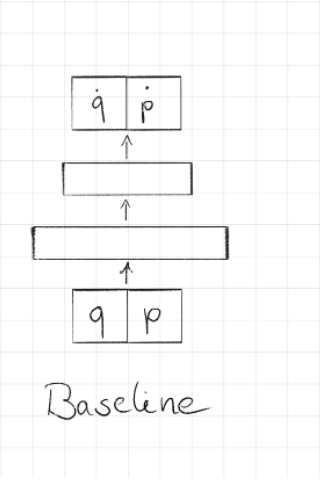
\includegraphics[width=0.6\textwidth]{baseline_nn_scheme.png}
			\caption{Схема работы базового решения моделирования динамики физической системы нейронными сетями}
			\label{fig:y equals x}
		\end{subfigure}
		\hfill
		\begin{subfigure}[b]{0.49\textwidth}
			\centering
			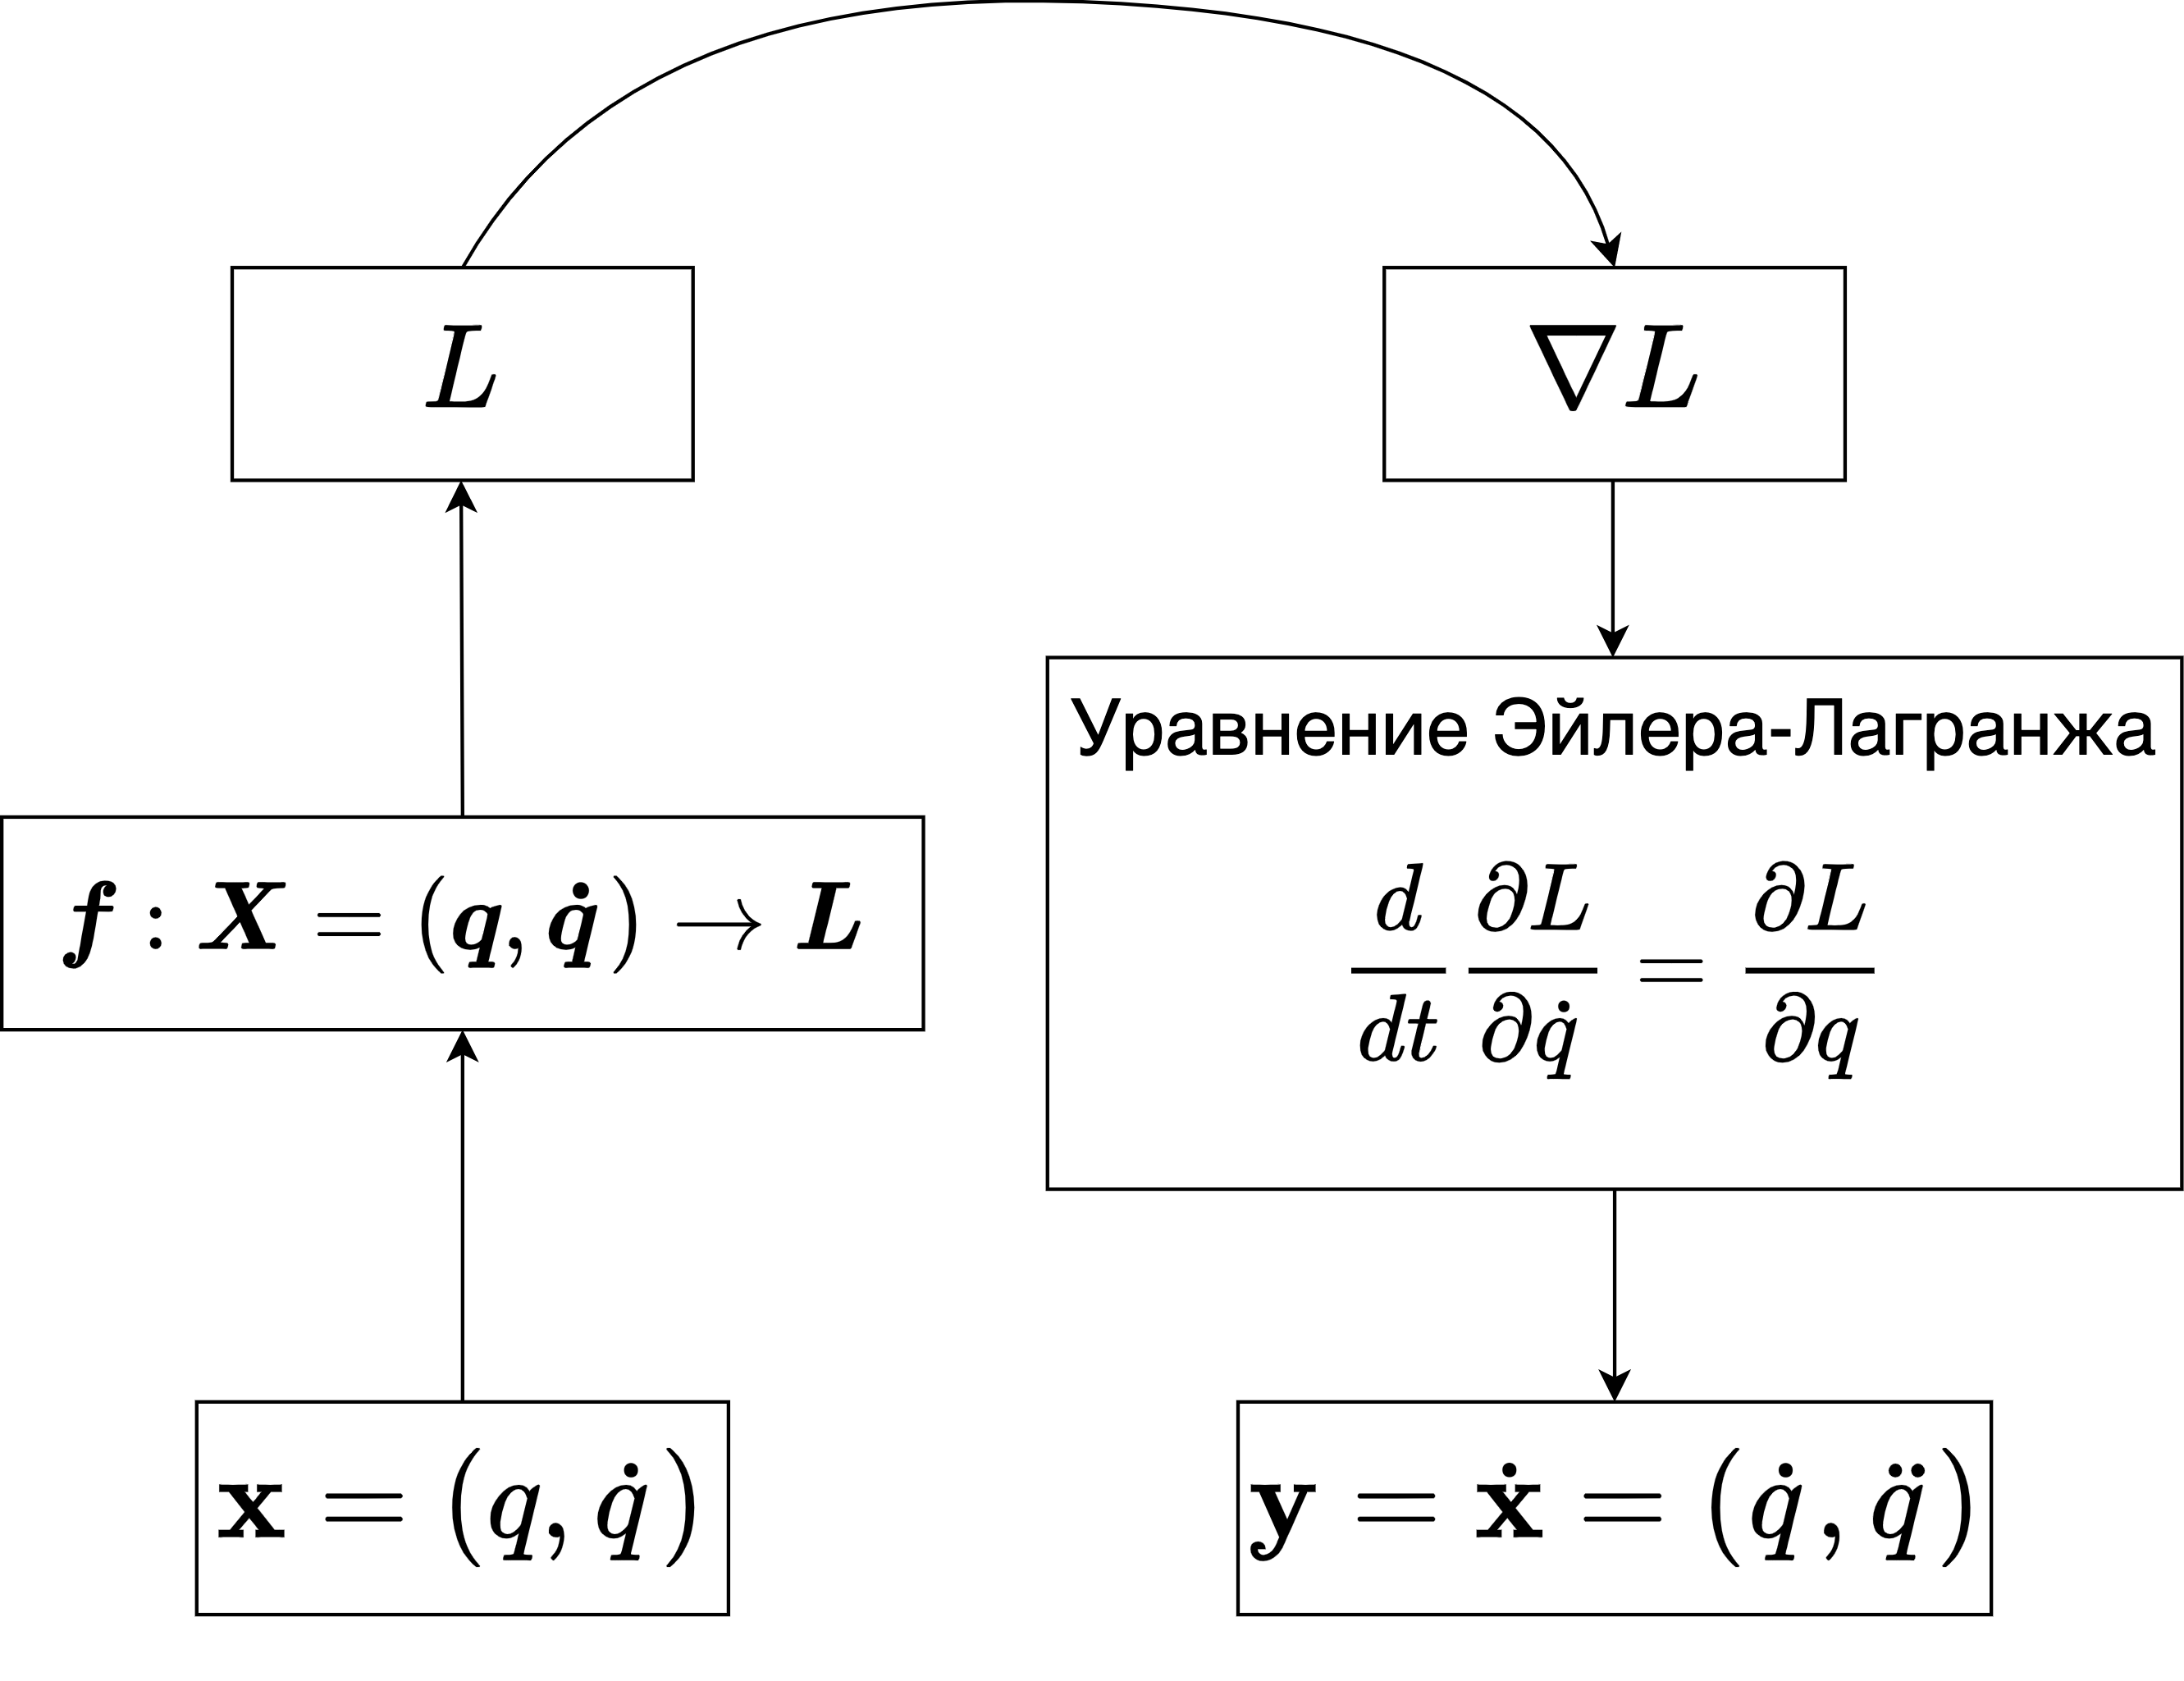
\includegraphics[width=\textwidth]{lnn_scheme.png}
			\caption{Схема работы Lagrangian Neural Networks (LNN) моделирования динамики физической системы}
			\label{fig:three sin x}
		\end{subfigure}
	\end{figure}

	
	\section{Теорема Нётер}
	\textbf{Определение 1 (Генераторы и инвариантность)}. Пусть $L(t, x,\dot{x})$ -- лагранжиан. Рассматривается преобразование 
	\begin{equation}
	\begin{aligned}
	t \mapsto t^{\prime} &=T(t, \boldsymbol{x}, \epsilon) \\
	\boldsymbol{x} \mapsto \boldsymbol{x}^{\prime} &=X(t, \boldsymbol{x}, \epsilon)
	\end{aligned}
	\end{equation}
	где преобразование является гладким как функция от $\epsilon$ и при $\epsilon= 0$ является тождественным и. Пусть
	\begin{equation}
	\begin{array}{l}
	T(t, \boldsymbol{x}, \epsilon)=t+\tau(t, \boldsymbol{x}) \epsilon+O\left(\epsilon^{2}\right) \\
	X(t, \boldsymbol{x}, \epsilon)=\boldsymbol{x}+\xi(t, \boldsymbol{x}) \epsilon+O\left(\epsilon^{2}\right)
	\end{array}
	\end{equation}
	Члены $\tau (t, x)$ и $\xi (t, x)$ называются генераторами преобразования. Генератор оставляет Лагранжиан инвариантным, если
	\begin{equation}
	\mathcal{L}\left(t^{\prime}, \boldsymbol{x}^{\prime}, \dot{x}^{\prime}\right) \frac{d t^{\prime}}{d t}-\mathcal{L}(t, \boldsymbol{x}, \dot{\boldsymbol{x}})=O\left(\epsilon^{2}\right)
	\end{equation}
	
	\textbf{Теорема 1 (Закон сохранения Нётер)}.
	Пусть $\mathcal{L}(t, \boldsymbol{x}, \dot{\boldsymbol{x}})$ -- лагранжиан, инвариантный относительно генераторов $\tau(t, \boldsymbol{x})$ и $\boldsymbol{\xi}(t, \boldsymbol{x})$. Пусть $\boldsymbol{x}(t)$ -- экстремальная функция $J[\boldsymbol{x}]=\int \mathcal{L}(t, \boldsymbol{x}, \dot{\boldsymbol{x}}) d t$. Тогда
	$$
	\left\langle\frac{\partial \mathcal{L}}{\partial \dot{x}}, \boldsymbol{\xi}\right\rangle+\left(\mathcal{L}-\left\langle\dot{\boldsymbol{x}}, \frac{\partial \mathcal{L}}{\partial \dot{\boldsymbol{x}}}\right\rangle\right) \tau
	$$
	сохраняется по $\boldsymbol{x}(t)$.
	%\textbf{Сравнение}
	%	\begin{figure}[h]
	%		\centering
	%		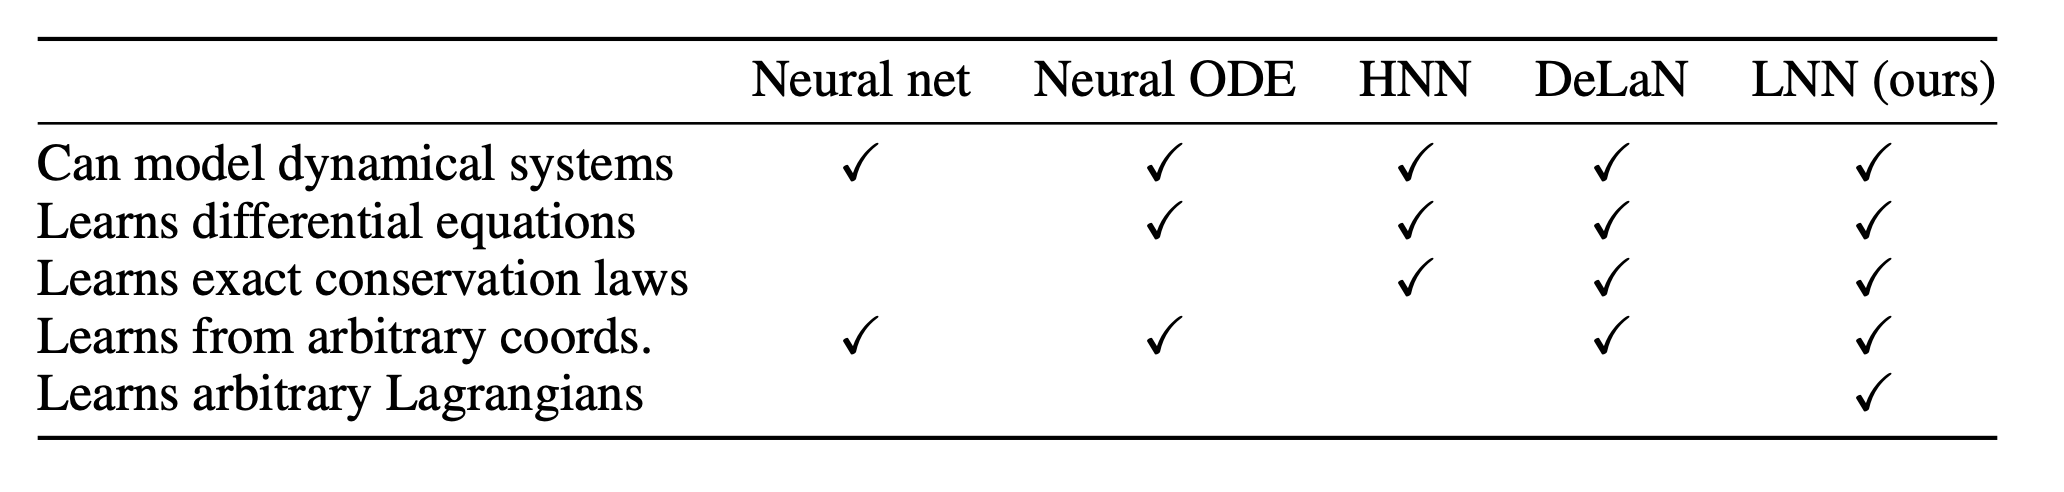
\includegraphics[width=1.05\textwidth]{comparison.png}
	%		\caption{Сравнение подходов моделирования физических систем нейронными сетями}
	%	\end{figure}
	
	
	%\subsection{Сверточные лагранжевы нейронные сети}
	%Добавление сверточных слоев в LNN/DeLaN
	
	\section{Вычислительный эксперимент}
	В рамках вычислительного эксперимента написан программный комплекс для решения поставленных задач~\cite{source_code}.
	
	\subsection{Постановка задачи}
	
	Пусть дана выборка $(\bX, \bY)$, где $\textbf{X} = [\textbf{x}_1, \dots, \textbf{x}_{n}]^{\T} \in \mathbb{R}^{n \times m}$~--- матрица независимых переменных, $\textbf{Y} = [\textbf{y}_1, \dots, \textbf{y}_n]^{\T} \in \mathbb{R}^{n \times k}$~--- матрица целевых переменных.
	
	\subsection{Данные: система двойного маятника}
	
	В качестве моделируемой физической системы взята система двойного маятника (Рис. \ref{fig:pendulum_system}). Двойной маятник образуется путем присоединения одного маятника к другому. Каждый маятник состоит из груза, соединенного с безмассовым жестким стержнем, который может двигаться только в вертикальной плоскости. Ось первого маятника закреплена в точке $O$. Все движения без трения.
	
	\begin{figure}[H]
			\centering
			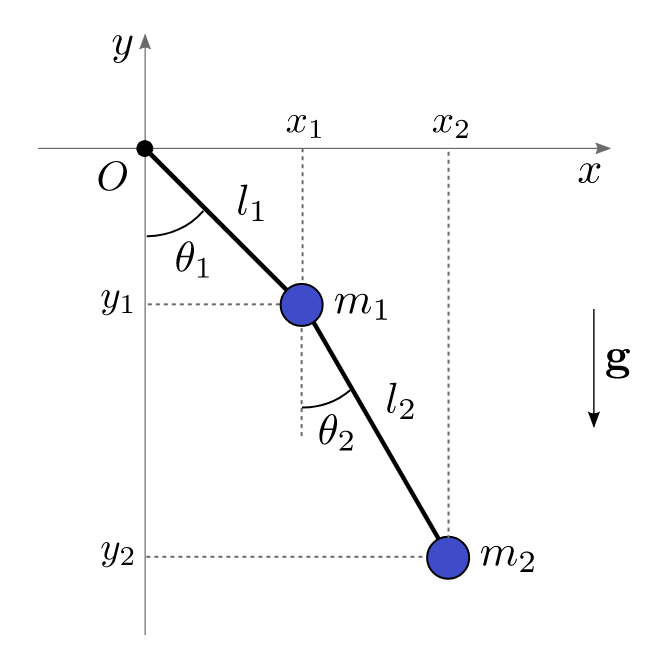
\includegraphics[width=0.4\textwidth]{double_pendulum_scheme.png}
			\caption{Cхема физической системы двойного маятника}
			\label{fig:pendulum_system}
	\end{figure}
	\begin{figure}[H]
	\centering
	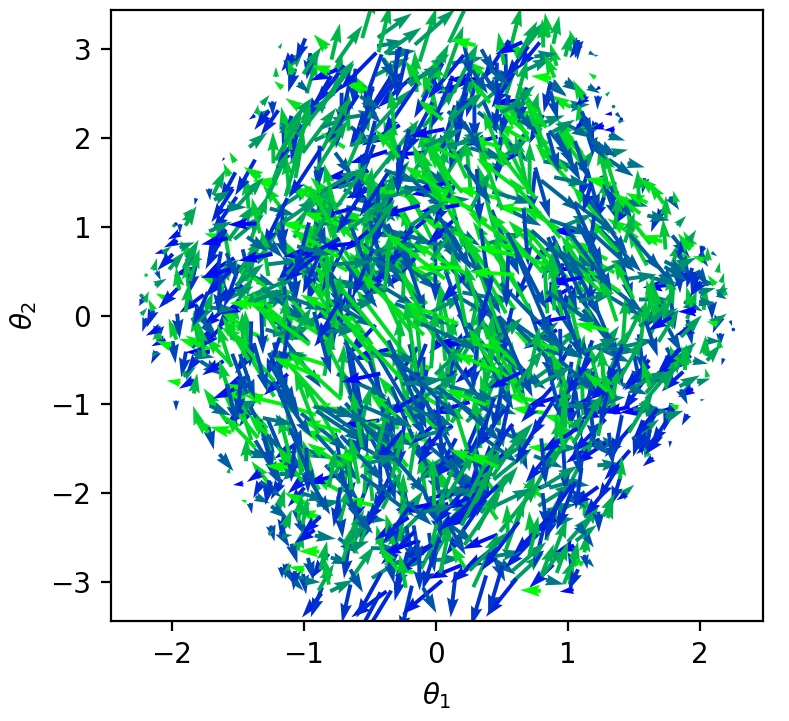
\includegraphics[width=0.9\textwidth]{train_test_data_vis.png}
	\caption{Визуализация данных канонических координат системы двойного маятника}
	\label{fig:canon}
\end{figure}

	\subsubsection{Лагранжиан системы}
	
	Примем точку $O$ за начало декартовой системы координат с осью $x$, направленной вдоль горизонтального направления, и осью $y$, направленной вертикально вверх. Пусть $\theta_1$ и $\theta_2$ -- углы, которые первый и второй стержни образуют с вертикальным направлением соответственно. Как видно на рисунке \ref{fig:pendulum_system}, положения грузов задаются следующим образом:
	
	$$
	\begin{aligned}
	x_{1} & =l_{1} \sin \theta_{1}, && y_{1}=-l_{1} \cos \theta_{1}, \\
	x_{2} & =l_{1} \sin \theta_{1}+l_{2} \sin \theta_{2}, &&  y_{2}=-l_{1} \cos \theta_{1}-l_{2} \cos \theta_{2}
	\end{aligned}
	$$
	
	Дифференцируя приведенные выше величины по времени, получаем скорости грузов:
	
	$$
	\begin{aligned}
	\dot{x}_{1} &=l_{1} \dot{\theta}_{1} \cos \theta_{1} & & \dot{y}_{1}=l_{1} \dot{\theta}_{1} \sin \theta_{1} \\
	\dot{x}_{2} &=l_{1} \dot{\theta}_{1} \cos \theta_{1}+l_{2} \dot{\theta}_{2} \cos \theta_{2} & & \dot{y}_{2}=l_{1} \dot{\theta}_{1} \sin \theta_{1}+l_{2} \dot{\theta}_{2} \sin \theta_{2}
	\end{aligned}
	$$
	
	Данная система имеет лагранжиан:
	$$
	\begin{aligned}
	L=\frac{1}{2}\left(m_{1}+m_{2}\right) l_{1}^{2} \dot{\theta}_{1}^{2} &+\frac{1}{2} m_{2} l_{2}^{2} \dot{\theta}_{2}^{2}+m_{2} l_{1} l_{2} \dot{\theta}_{1} \dot{\theta}_{2} \cos \left(\theta_{1}-\theta_{2}\right) \\
	&+\left(m_{1}+m_{2}\right) g l_{1} \cos \theta_{1}+m_{2} g l_{2} \cos \theta_{2}
	\end{aligned}
	$$
	
	Лагранжиан для двойного маятника определяется выражением $L=T - V$, где $T$ и $V$ -- кинетическая и потенциальная энергии системы соответственно. Кинетическая энергия $T$ определяется выражением:
	$$
	\begin{aligned}
	T &=\frac{1}{2} m_{1} v_{1}^{2}+\frac{1}{2} m_{2} v_{2}^{2} \\
	&=\frac{1}{2} m_{1}\left(\dot{x}_{1}^{2}+\dot{y}_{1}^{2}\right)+\frac{1}{2} m_{2}\left(\dot{x}_{2}^{2}+\dot{y}_{2}^{2}\right) \\
	&=\frac{1}{2} m_{1} l_{1}^{2} \dot{\theta}_{1}^{2}+\frac{1}{2} m_{2}\left[l_{1}^{2} \dot{\theta}_{1}^{2}+l_{2}^{2} \dot{\theta}_{2}^{2}+2 l_{1} l_{2} \dot{\theta}_{1} \dot{\theta}_{2} \cos \left(\theta_{1}-\theta_{2}\right)\right]
	\end{aligned}
	$$
	
	В выражении выше использован факт, что $\cos \theta_{1} \cos \theta_{2}+\sin \theta_{1} \sin \theta_{2}=\cos \left(\theta_{1}-\theta_{2}\right)$. Потенциальная энергия $V$ определяется выражением:
	$$
	\begin{aligned}
	V &=m_{1} g y_{1}+m_{2} g y_{2} \\
	&=-m_{1} g l_{1} \cos \theta_{1}-m_{2} g\left(l_{1} \cos \theta_{1}+l_{2} \cos \theta_{2}\right) \\
	&=-\left(m_{1}+m_{2}\right) g l_{1} \cos \theta_{1}-m_{2} g l_{2} \cos \theta_{2}
	\end{aligned}
	$$
	Таким образом, Лагранжиан системы:
	$$
	\begin{aligned}
	L=\frac{1}{2}\left(m_{1}+m_{2}\right) l_{1}^{2} \dot{\theta}_{1}^{2} &+\frac{1}{2} m_{2} l_{2}^{2} \dot{\theta}_{2}^{2}+m_{2} l_{1} l_{2} \dot{\theta}_{1} \dot{\theta}_{2} \cos \left(\theta_{1}-\theta_{2}\right) \\
	&+\left(m_{1}+m_{2}\right) g l_{1} \cos \theta_{1}+m_{2} g l_{2} \cos \theta_{2}
	\end{aligned}
	$$
	
	Исходя из данного лагранжиана получаем канонические координаты системы (Рис. \ref{fig:canon})

	\subsubsection{Аналитическое решение получения динамики системы}
	The canonical momenta associated with the coordinates $\theta_{1}$ and $\theta_{2}$ can be obtained directly from $L$ :
	$$
	\begin{array}{l}
	p_{\theta_{1}}=\frac{\partial L}{\partial \dot{\theta}_{1}}=\left(m_{1}+m_{2}\right) l_{1}^{2} \dot{\theta}_{1}+m_{2} l_{1} l_{2} \dot{\theta}_{2} \cos \left(\theta_{1}-\theta_{2}\right) \\
	p_{\theta_{2}}=\frac{\partial L}{\partial \dot{\theta}_{2}}=m_{2} l_{2}^{2} \dot{\theta}_{2}+m_{2} l_{1} l_{2} \dot{\theta}_{1} \cos \left(\theta_{1}-\theta_{2}\right)
	\end{array}
	$$
	The equations of motion of the system are the Euler-Lagrange equations:
	$$
	\frac{d}{d t}\left(\frac{\partial L}{\partial \dot{\theta}_{i}}\right)-\frac{\partial L}{\partial \theta_{i}}=0 \Longrightarrow \frac{d p_{\theta_{i}}}{d t}-\frac{\partial L}{\partial \theta_{i}}=0 \quad \text { for } \quad i=1,2
	$$
	Since:
	$$
	\begin{aligned}
	\frac{d p_{\theta_{1}}}{d t}=&\left(m_{1}+m_{2}\right) l_{1}^{2} \ddot{\theta}_{1}+m_{2} l_{1} l_{2} \ddot{\theta}_{2} \cos \left(\theta_{1}-\theta_{2}\right) \\
	&-m_{2} l_{1} l_{2} \dot{\theta}_{2} \dot{\theta}_{1} \sin \left(\theta_{1}-\theta_{2}\right)+m_{2} l_{1} l_{2} \dot{\theta}_{2}^{2} \sin \left(\theta_{1}-\theta_{2}\right) \\
	\frac{d p_{\theta_{2}}}{d t}=& m_{2} l_{2}^{2} \ddot{\theta}_{2}+m_{2} l_{1} l_{2} \ddot{\theta}_{1} \cos \left(\theta_{1}-\theta_{2}\right) \\
	& \quad-m_{2} l_{1} l_{2} \dot{\theta}_{1}^{2} \sin \left(\theta_{1}-\theta_{2}\right)+m_{2} l_{1} l_{2} \dot{\theta}_{1} \dot{\theta}_{2} \sin \left(\theta_{1}-\theta_{2}\right) \\
	\frac{\partial L}{\partial \theta_{1}}=&-m_{2} l_{1} l_{2} \dot{\theta}_{1} \dot{\theta}_{2} \sin \left(\theta_{1}-\theta_{2}\right)-\left(m_{1}+m_{2}\right) g l_{1} \sin \theta_{1} \\
	\frac{\partial L}{\partial \theta_{2}}=& m_{2} l_{1} l_{2} \dot{\theta}_{1} \dot{\theta}_{2} \sin \left(\theta_{1}-\theta_{2}\right)-m_{2} g l_{2} \sin \theta_{2}
	\end{aligned}
	$$
	then equation (10) yields (after dividing by $l_{1}$ when $i=1$ and by $m_{2} l_{2}$ when $i=2$ ):
	$$
	\begin{aligned}
	\left(m_{1}+m_{2}\right) l_{1} \ddot{\theta}_{1} &+m_{2} l_{2} \ddot{\theta}_{2} \cos \left(\theta_{1}-\theta_{2}\right) \\
	&+m_{2} l_{2} \dot{\theta}_{2}^{2} \sin \left(\theta_{1}-\theta_{2}\right)+\left(m_{1}+m_{2}\right) g \sin \theta_{1}=0
	\end{aligned}
	$$
	$l_{2} \ddot{\theta}_{2}+l_{1} \ddot{\theta}_{1} \cos \left(\theta_{1}-\theta_{2}\right)-l_{1} \dot{\theta}_{1}^{2} \sin \left(\theta_{1}-\theta_{2}\right)+g \sin \theta_{2}=0$
	
	The canonical momenta associated with the coordinates $\theta_{1}$ and $\theta_{2}$ can be obtained directly from $L$ :
	$$
	\begin{array}{l}
	p_{\theta_{1}}=\frac{\partial L}{\partial \dot{\theta}_{1}}=\left(m_{1}+m_{2}\right) l_{1}^{2} \dot{\theta}_{1}+m_{2} l_{1} l_{2} \dot{\theta}_{2} \cos \left(\theta_{1}-\theta_{2}\right) \\
	p_{\theta_{2}}=\frac{\partial L}{\partial \dot{\theta}_{2}}=m_{2} l_{2}^{2} \dot{\theta}_{2}+m_{2} l_{1} l_{2} \dot{\theta}_{1} \cos \left(\theta_{1}-\theta_{2}\right)
	\end{array}
	$$
	The equations of motion of the system are the Euler-Lagrange equations:
	$$
	\frac{d}{d t}\left(\frac{\partial L}{\partial \dot{\theta}_{i}}\right)-\frac{\partial L}{\partial \theta_{i}}=0 \Longrightarrow \frac{d p_{\theta_{i}}}{d t}-\frac{\partial L}{\partial \theta_{i}}=0 \quad \text { for } \quad i=1,2
	$$
	Since:
	$$
	\begin{aligned}
	\frac{d p_{\theta_{1}}}{d t}=&\left(m_{1}+m_{2}\right) l_{1}^{2} \ddot{\theta}_{1}+m_{2} l_{1} l_{2} \ddot{\theta}_{2} \cos \left(\theta_{1}-\theta_{2}\right) \\
	&-m_{2} l_{1} l_{2} \dot{\theta}_{2} \dot{\theta}_{1} \sin \left(\theta_{1}-\theta_{2}\right)+m_{2} l_{1} l_{2} \dot{\theta}_{2}^{2} \sin \left(\theta_{1}-\theta_{2}\right) \\
	\frac{d p_{\theta_{2}}}{d t}=& m_{2} l_{2}^{2} \ddot{\theta}_{2}+m_{2} l_{1} l_{2} \ddot{\theta}_{1} \cos \left(\theta_{1}-\theta_{2}\right) \\
	& \quad-m_{2} l_{1} l_{2} \dot{\theta}_{1}^{2} \sin \left(\theta_{1}-\theta_{2}\right)+m_{2} l_{1} l_{2} \dot{\theta}_{1} \dot{\theta}_{2} \sin \left(\theta_{1}-\theta_{2}\right) \\
	\frac{\partial L}{\partial \theta_{1}}=&-m_{2} l_{1} l_{2} \dot{\theta}_{1} \dot{\theta}_{2} \sin \left(\theta_{1}-\theta_{2}\right)-\left(m_{1}+m_{2}\right) g l_{1} \sin \theta_{1} \\
	\frac{\partial L}{\partial \theta_{2}}=& m_{2} l_{1} l_{2} \dot{\theta}_{1} \dot{\theta}_{2} \sin \left(\theta_{1}-\theta_{2}\right)-m_{2} g l_{2} \sin \theta_{2}
	\end{aligned}
	$$
	then equation (10) yields (after dividing by $l_{1}$ when $i=1$ and by $m_{2} l_{2}$ when $i=2$ ):
	$$
	\begin{aligned}
	\left(m_{1}+m_{2}\right) l_{1} \ddot{\theta}_{1} &+m_{2} l_{2} \ddot{\theta}_{2} \cos \left(\theta_{1}-\theta_{2}\right) \\
	&+m_{2} l_{2} \dot{\theta}_{2}^{2} \sin \left(\theta_{1}-\theta_{2}\right)+\left(m_{1}+m_{2}\right) g \sin \theta_{1}=0
	\end{aligned}
	$$
	$l_{2} \ddot{\theta}_{2}+l_{1} \ddot{\theta}_{1} \cos \left(\theta_{1}-\theta_{2}\right)-l_{1} \dot{\theta}_{1}^{2} \sin \left(\theta_{1}-\theta_{2}\right)+g \sin \theta_{2}=0$
	
	Equations $(15)$ and $(16)$ form a system of coupled second-order nonlinear differential equations. Dividing equation $(15)$ by $\left(m_{1}+m_{2}\right) l_{1}$ and equation (16) by $l_{2}$ and also moving all terms which do not involve $\ddot{\theta}_{1}$ and $\ddot{\theta}_{2}$ to the right-hand side, we obtain:
	$$
	\begin{array}{l}
	\ddot{\theta}_{1}+\alpha_{1}\left(\theta_{1}, \theta_{2}\right) \ddot{\theta}_{2}=f_{1}\left(\theta_{1}, \theta_{2}, \dot{\theta}_{1}, \dot{\theta}_{2}\right) \\
	\ddot{\theta}_{2}+\alpha_{2}\left(\theta_{1}, \theta_{2}\right) \ddot{\theta}_{1}=f_{2}\left(\theta_{1}, \theta_{2}, \dot{\theta}_{1}, \dot{\theta}_{2}\right)
	\end{array}
	$$
	where:
	$$
	\begin{array}{l}
	\alpha_{1}\left(\theta_{1}, \theta_{2}\right):=\frac{l_{2}}{l_{1}}\left(\frac{m_{2}}{m_{1}+m_{2}}\right) \\
	\alpha_{2}\left(\theta_{1}, \theta_{2}\right):=\frac{l_{1}}{l_{2}} \cos \left(\theta_{1}-\theta_{2}\right)
	\end{array}
	$$
	and:
	$$
	\begin{array}{l}
	f_{1}\left(\theta_{1}, \theta_{2}, \dot{\theta}_{1}, \dot{\theta}_{2}\right):=-\frac{l_{2}}{l_{1}}\left(\frac{m_{2}}{m_{1}+m_{2}}\right) \dot{\theta}_{2}^{2} \sin \left(\theta_{1}-\theta_{2}\right)-\frac{g}{l_{1}} \sin \theta_{1} \\
	f_{2}\left(\theta_{1}, \theta_{2}, \dot{\theta}_{1}, \dot{\theta}_{2}\right):=\frac{l_{1}}{l_{2}} \dot{\theta}_{1}^{2} \sin \left(\theta_{1}-\theta_{2}\right)-\frac{g}{l_{2}} \sin \theta_{2}
	\end{array}
	$$
	Interestingly, $f_{1}$ does not depent on $\dot{\theta}_{1}$ and $f_{2}$ does not depend on $\dot{\theta}_{2}$. Equations (17) and (18) can be combined into a single equation:
	$$
	A\left(\begin{array}{l}
	\ddot{\theta}_{1} \\
	\ddot{\theta}_{2}
	\end{array}\right)=\left(\begin{array}{cc}
	1 & \alpha_{1} \\
	\alpha_{2} & 1
	\end{array}\right)\left(\begin{array}{c}
	\ddot{\theta}_{1} \\
	\ddot{\theta}_{2}
	\end{array}\right)=\left(\begin{array}{l}
	f_{1} \\
	f_{2}
	\end{array}\right)
	$$
	where the matrix $A$ depends on $\theta_{1}$ and $\theta_{2}$ since $\alpha_{1}$ and $\alpha_{2}$ depend on these variables. Being a $2 \times 2$ matrix, $A$ can be inverted directly:
	$$
	A^{-1}=\frac{1}{\operatorname{det}(A)}\left(\begin{array}{cc}
	1 & -\alpha_{1} \\
	-\alpha_{2} & 1
	\end{array}\right)=\frac{1}{1-\alpha_{1} \alpha_{2}}\left(\begin{array}{cc}
	1 & -\alpha_{1} \\
	-\alpha_{2} & 1
	\end{array}\right)
	$$
	Before we continue, notice that $A$ is always invertible since:
	$$
	\operatorname{det}(A)=1-\alpha_{1} \alpha_{2}=1-\left(\frac{m_{2}}{m_{1}+m_{2}}\right) \cos ^{2}\left(\theta_{1}-\theta_{2}\right)>0
	$$
	because $m_{2} /\left(m_{1}+m_{2}\right)<1$ and $\cos ^{2}(x) \leq 1$ for all real values of $x$. From equations $(23)$ and (24) we obtain:
	$$
	\left(\begin{array}{l}
	\ddot{\theta}_{1} \\
	\ddot{\theta}_{2}
	\end{array}\right)=A^{-1}\left(\begin{array}{l}
	f_{1} \\
	f_{2}
	\end{array}\right)=\frac{1}{1-\alpha_{1} \alpha_{2}}\left(\begin{array}{c}
	f_{1}-\alpha_{1} f_{2} \\
	-\alpha_{2} f_{1}+f_{2}
	\end{array}\right)
	$$
	Finally, letting $\omega_{1}:=\dot{\theta}_{1}$ and $\omega_{2}:=\dot{\theta}_{2}$, we can write the equations of motion of the double pendulum as a system of coupled first order differential equations on the variables $\theta_{1}, \theta_{2}, \omega_{1}$, $\omega_{2}:$
	$$
	\begin{array}{c}
	\frac{d}{d t}\left(\begin{array}{c}
	\theta_{1} \\
	\theta_{2} \\
	\omega_{1} \\
	\omega_{1}
	\end{array}\right)=\left(\begin{array}{c}
	\omega_{1} \\
	\omega_{2} \\
	g_{1}\left(\theta_{1}, \theta_{2}, \omega_{1}, \omega_{2}\right) \\
	g_{2}\left(\theta_{1}, \theta_{2}, \omega_{1}, \omega_{2}\right)
	\end{array}\right) \\
	g_{1}:=\frac{f_{1}-\alpha_{1} f_{2}}{1-\alpha_{1} \alpha_{2}} \quad g_{2}:=\frac{-\alpha_{2} f_{1}+f_{2}}{1-\alpha_{1} \alpha_{2}}
	\end{array}
	$$
	where $\alpha_{i}=\alpha_{i}\left(\theta_{1}, \theta_{2}\right)$ and $f_{i}=f_{i}\left(\theta_{1}, \theta_{2}, \omega_{1}, \omega_{2}\right)$ for $i=1,2$ are given on equations (19)(22).
	
	Equation (27) can be solved numerically using a Runge-Kutta (RK) method. A simulator based on the fourth-order RK method can be found here.
	
	\subsection{Исследуемые модели нейронных сетей}
	\subsubsection{Полносвязная нейронная сеть}
	\begin{equation}
	f_{\boldsymbol{w}}(\boldsymbol{x}):=\sigma_{K}\left(W^{(K)} \sigma_{K-1}\left(W^{(K-1)} \cdots \sigma_{1}\left(W^{(1)} \boldsymbol{x}\right)\right)\right)
	\end{equation}
	
	\subsubsection{LSTM}
	\subsubsection{LNN}
	\subsubsection{LNN, учитывающая трансляционную и вращательную симметрии}
	\textbf{Нётеровская Лагранжева нейронная сеть}
	LNN, получающая на вход разницу между каноническими координатами $\delta \theta_{12} = \theta_1-\theta_2$ и аппроксимирующая потенциальную энергию системы $V(\delta \theta_{12})$
	
	
	Аппроксимируемый лагранжиан примет вид:
	$$
	L=\frac{1}{2}\left(m_{1}+m_{2}\right) l_{1}^{2} \dot{\theta}_{1}^{2} +\frac{1}{2} m_{2} l_{2}^{2} \dot{\theta}_{2}^{2}+m_{2} l_{1} l_{2} \dot{\theta}_{1} \dot{\theta}_{2} \cos \left(\delta \theta_{12}\right) + V(\delta \theta_{12})
	$$
	
	\textbf{Теорема 1}
	Нётеровская LNN учитывает трансляционную симметрию.
	\textbf{Доказательство}
	аааааа
	
	\textbf{Теорема 2}
	Нётеровская LNN учитывает вращательную симметрию.
	\textbf{Доказательство}
	аааааа

	\subsection{Результаты}
	Результаты моделирования динамики системы двойного маятника различными видами нейронных сетей представлены на рисунке \ref{fig:three graphs}
	
	\begin{table}[]
		\begin{tabular}{|l|l|l|l|l|}
			\hline
			& FC          & LSTM        & LNN         & Нётеровская LNN \\ \hline
			MSE & $0.00 \pm 0.01$ & $0.00 \pm 0.01$ & $0.00 \pm 0.01$ & \textbf{0.00} $ \pm 0.01$ \\ \hline
		\end{tabular}
		\caption{Средняя ошибка MSE между предсказанной динамикой системы нейронной сетью и динамикой системы, полученной аналитическим решением.}
	\end{table}

	\begin{figure}[H]
		\centering
		\begin{subfigure}[b]{0.49\textwidth}
			\centering
			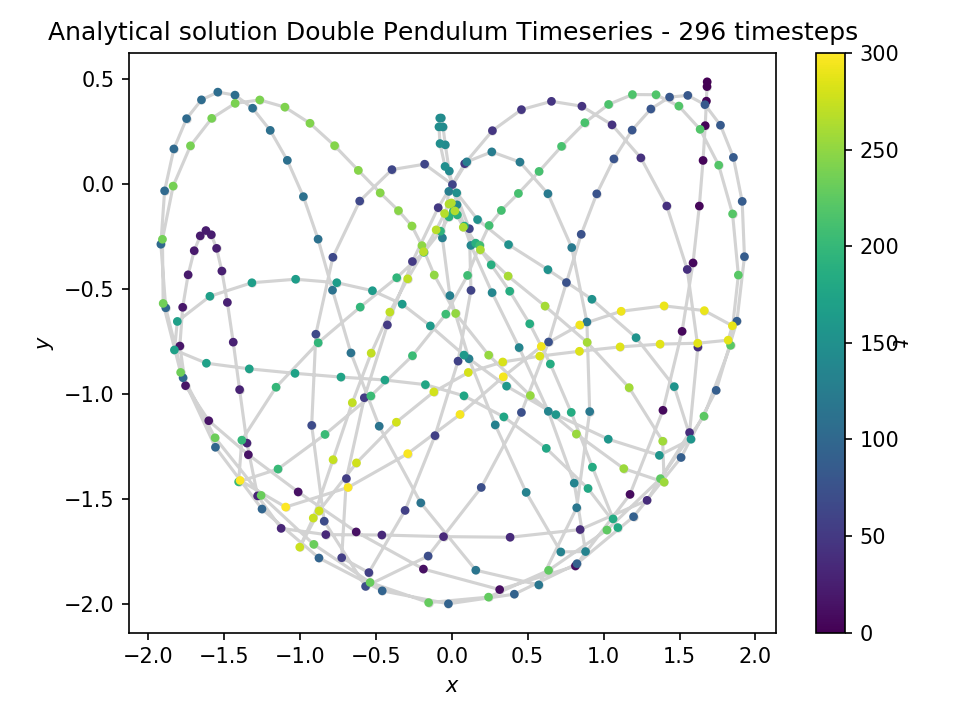
\includegraphics[width=\textwidth]{predicted_trajectory_Analytical solution.png}
			\caption{Аналитическое решение}
			\label{fig:y equals x}
		\end{subfigure}
		\hfill
		\begin{subfigure}[b]{0.49\textwidth}
			\centering
			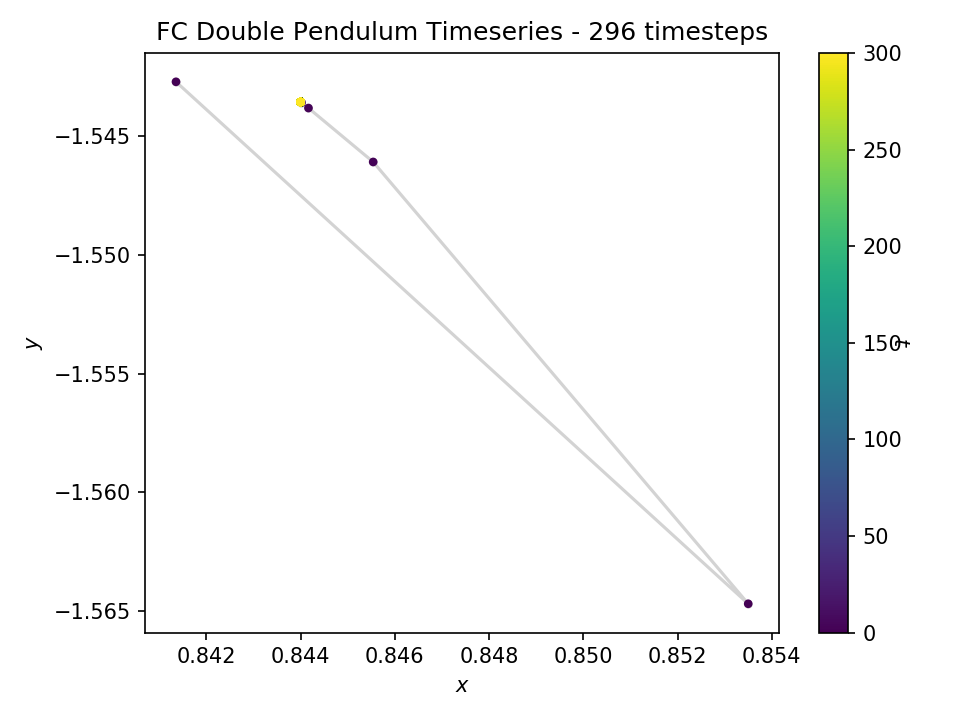
\includegraphics[width=\textwidth]{predicted_trajectory_FC.png}
			\caption{Динамика системы с помощью полносвязной нейронной сети}
			\label{fig:three sin x}
		\end{subfigure}
				\hfill
				\vfill
		\begin{subfigure}[b]{0.49\textwidth}
			\centering
			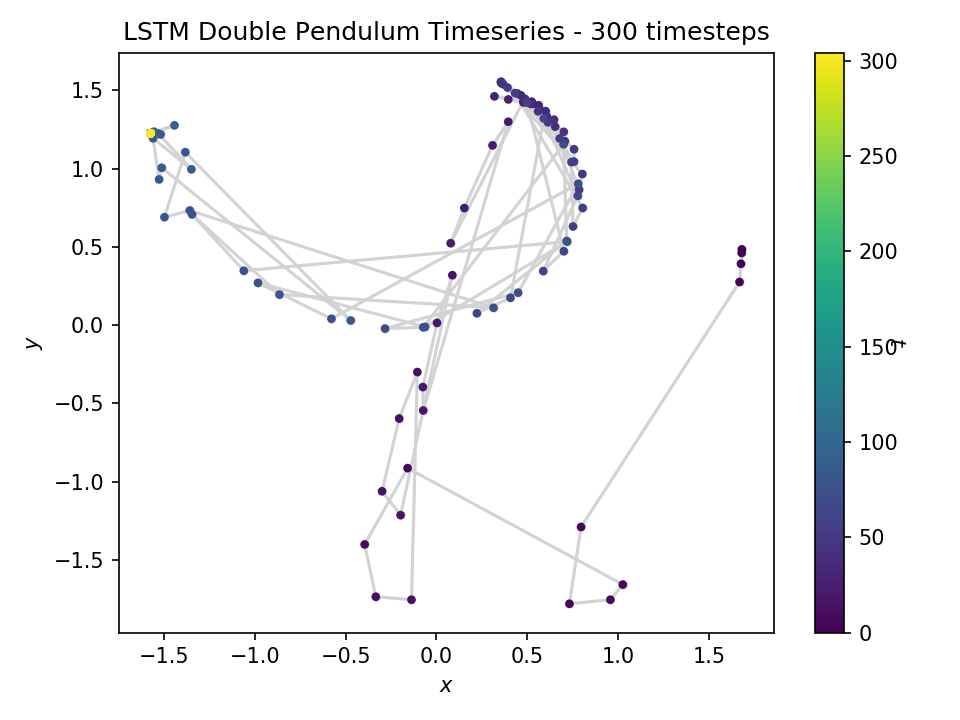
\includegraphics[width=\textwidth]{predicted_trajectory_LSTM.png}
			\caption{Динамика системы с помощью LSTM}
			\label{fig:three sin x}
		\end{subfigure}
			\hfill
		%\begin{subfigure}[b]{0.49\textwidth}
		%	\centering
		%	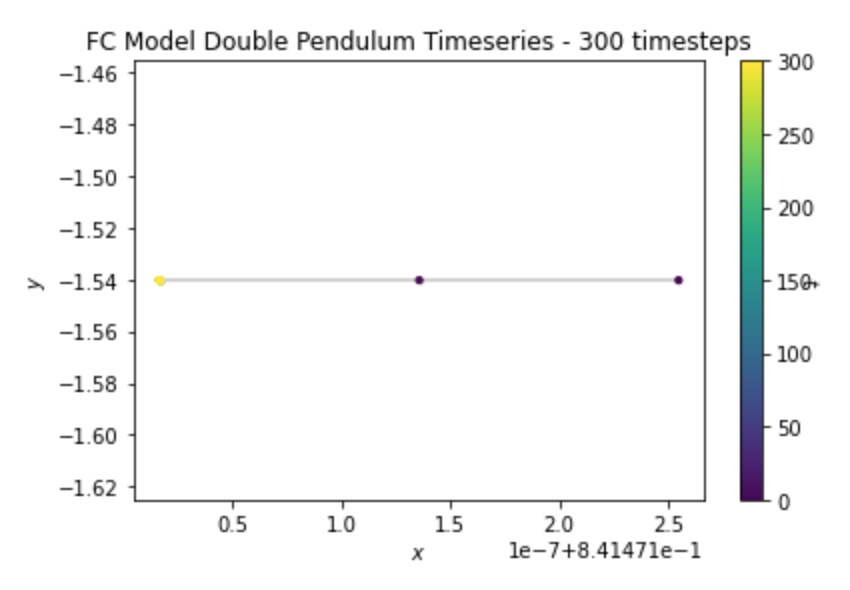
\includegraphics[width=\textwidth]{fc_pendulum.png}
		%	\caption{TODO Динамика системы с помощью Neural ODE}
		%	\label{fig:five over x}
		%\end{subfigure}
		\begin{subfigure}[b]{0.49\textwidth}
			\centering
			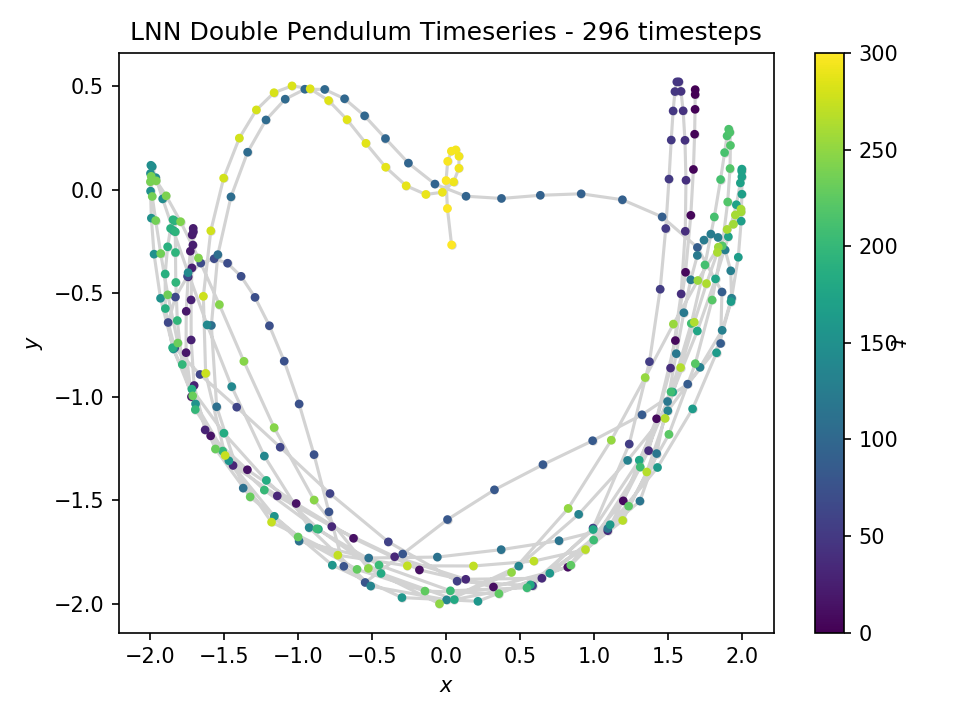
\includegraphics[width=\textwidth]{predicted_trajectory_LNN.png}
			\caption{Динамика системы с помощью LNN}
			\label{fig:five over x}
		\end{subfigure}
	\begin{subfigure}[b]{0.49\textwidth}
		\centering
		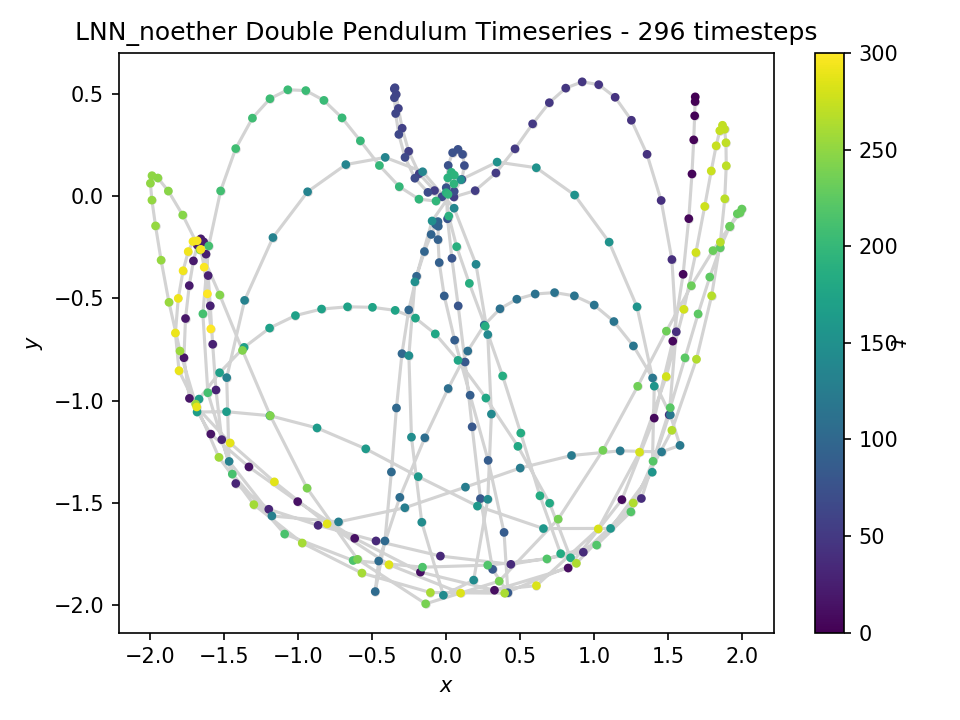
\includegraphics[width=\textwidth]{predicted_trajectory_LNN_noether.png}
		\caption{Динамика системы с помощью LNN}
		\label{fig:five over x}
	\end{subfigure}
		\caption{Моделирование динамики системы двойного маятника различными видами нейронных сетей: аналитическое решение, полносвязная нейронная сеть, LSTM, LNN.}
		\label{fig:three graphs}
	\end{figure}
	
	
	\section{Заключение}
	В работе рассмотрена задача 
	\begin{itemize}
		\item Показано, что LNN является оптимальной среди моделей FN, LSTM
		\item Представлена Нётеровская LNN, учитываящая дополнительные симметрии кроме закона сохранения энергии
		\item Показано, что более интерпретируемая модель дает более точные результаты для решения задачи моделирования динамики физической системы
	\end{itemize}
	\bibliographystyle{unsrt}
	\bibliography{Severilov2022MasterThesisCite.bib}

	%\bibliographystyle{unsrt}
	%\begin{thebibliography}{99}
		
	
	%	\bibitem{source_code}
%		\textit{Severilov}. Project source code is available at:~\url{https://github.com/severilov/BCI-thesis}, 2021.
	%\end{thebibliography}
	
\end{document}

